\chapter{PC-Software FOC Studio}
\label{ch:focstudio}

\section{Anforderungen und Bedienkonzept}
% docs/GUI_Entscheidungen.md
\offen{Text}

\section{Architektur}
% host/core (fochost, Qt-frei): Transporte Sim, CANable/gs_usb, SocketCAN, PCAN; Device
% host/studio (Qt 6 Widgets, Qwt); host/app (ImGui, Entwicklerwerkzeug)
% Entscheidung für Qwt nach Plot-Benchmark
\offen{Text, Architekturbild}

\section{Funktionen}
% Übersicht/Dashboard, Parameter (JSON-Import/-Export), Scope, Inbetriebnahme,
% Expertenmodus, Ereignisprotokoll, Deutsch/Englisch
\offen{Text, Screenshot}
% 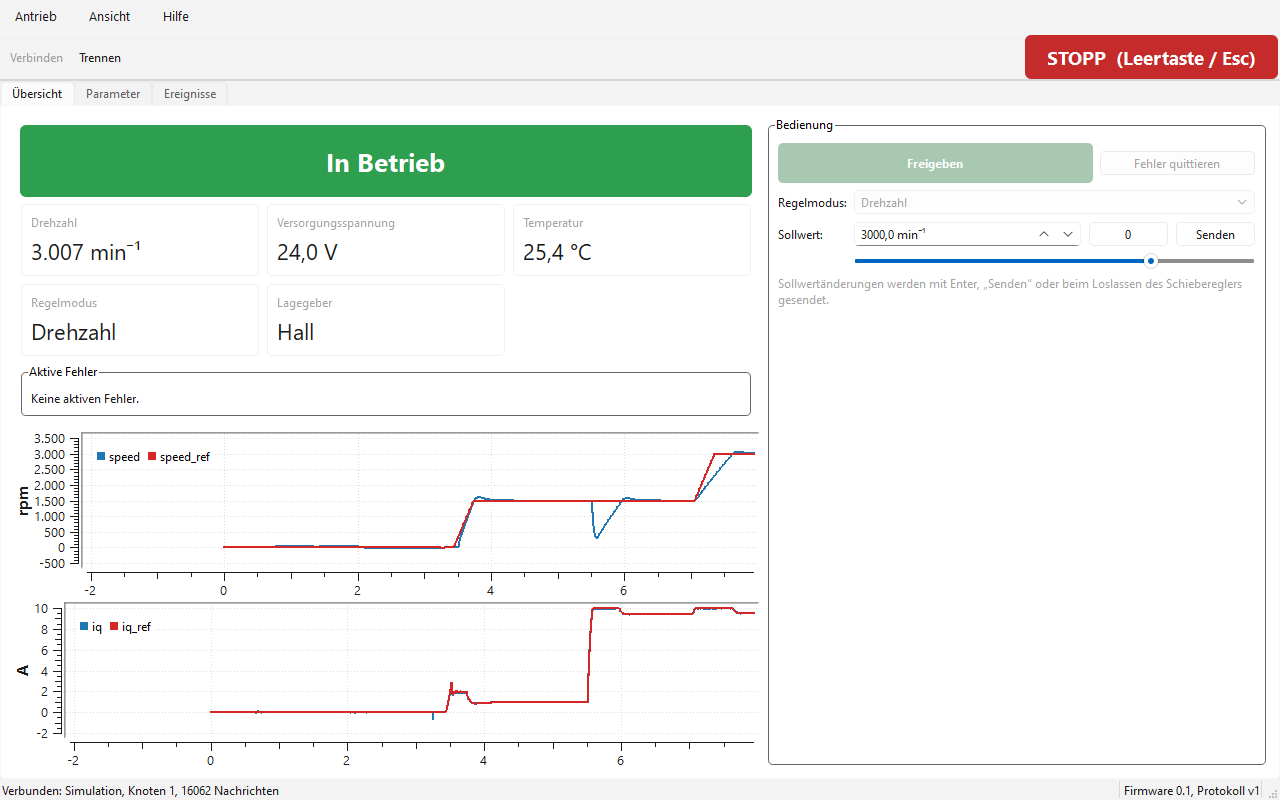
\includegraphics[width=\linewidth]{focstudio_dashboard}

\section{Tests und Auslieferung}
% ctest, virtueller Antrieb (--demo), Installer (NSIS/CPack)
\offen{Text}
